\subsection{Using a Language Model During Training}
\label{sec:trainwithlm}

A PT contains significant amount of information beyond any single
transcript extracted from the PT. Motivated by this, the statistics
for the MAP estimation are accumulated from a lattice derived from the
cascade $\mathbf{AM} \circ \mathbf{HC} \circ \mathbf{PT}$, rather than
reducing the PT to its single best path. Though it is disadvantageous
to reduce a PT to its best path, it is nevertheless advantageous to
incorporate as much information as possible from the language model
during adaptation.  Define $\mathbf{G}$ to be an FST representing the
modeled phone bigram probability
$\pi(\phi^\ell|\theta)=\prod_{m=1}^M\pi(\phi_m^\ell|\phi_{m-1}^\ell,\theta)$.
By assumption, such information is not available from speech: we
assume that there is no transcribed speech in the target language.  A
reasonable proxy, however, can be constructed from text.

\begin{figure}
  \centerline{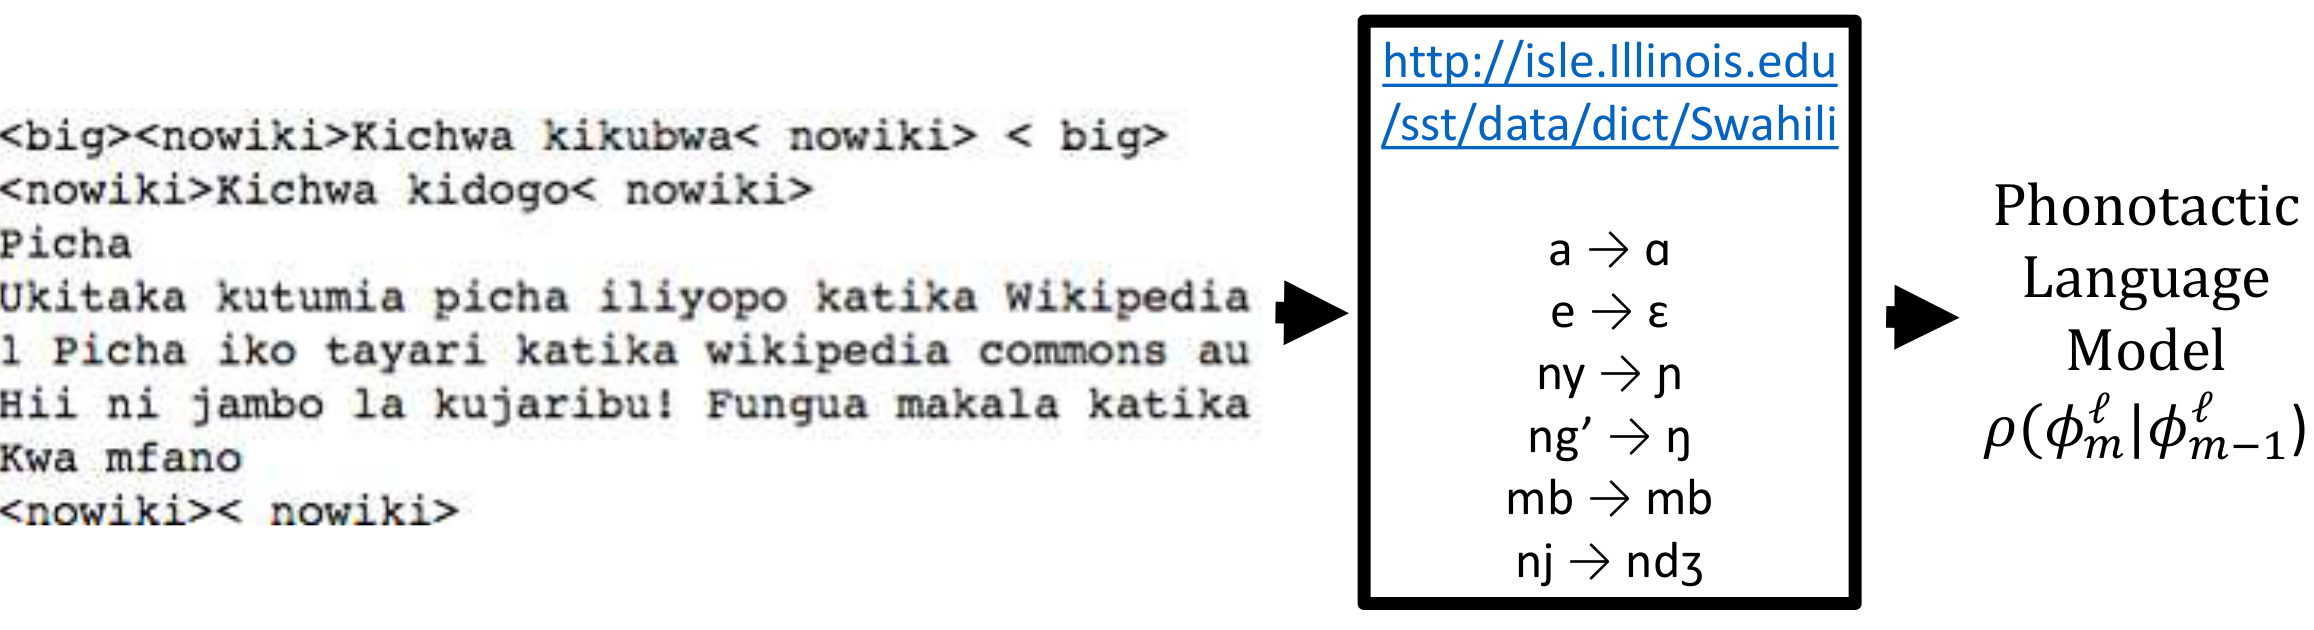
\includegraphics[width=5in]{../figs/fig_sloan.png}}
  \caption{A phonotactic language model (a bigram language model over
    phone sequences) can be trained using text data downloaded from
    Wikipedia (left), then converted into phone strings in the target
    language using a simple character-based grapheme-to-phoneme
    transducer (center).  In this example, the target language is
    Swahili.}
  \label{fig:wikitext}
\end{figure}

Fig.~\ref{fig:wikitext} shows text data downloaded from wikipedia in
Swahili, and a segment of a rule-based, character-by-character G2P for
the Swahili language~\cite{Hasegawajohnson15}.  By passing the former
through the latter, it is possible to generate synthetic phoneme
sequences in the target language.

\begin{figure}
  \centerline{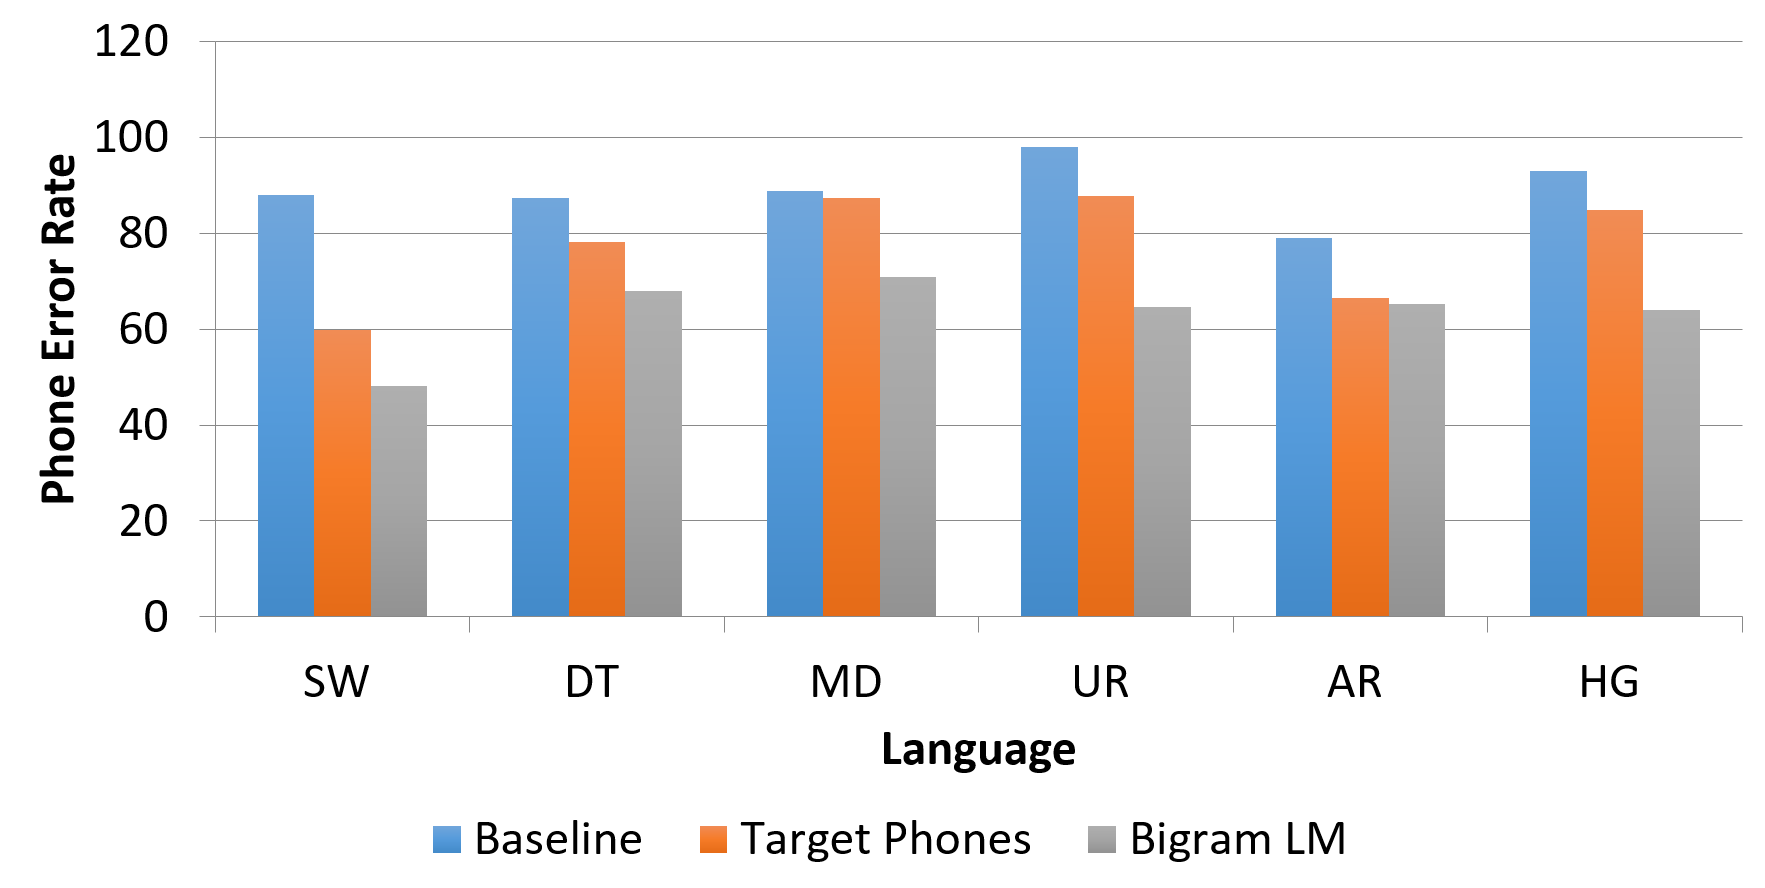
\includegraphics[width=4in]{../figs/sloan2.png}}
  \caption{PER of the 1-best path: a measure of the quality of
    probabilistic transcriptions acquired from mismatched
    crowdsourcing.  Native transcriptions were available in six
    languages: Swahili (SW), Dutch (DT), Mandarin (MN), Urdu (UR),
    Arabic (AR), and Hungarian (HG).  Probabilistic transcriptions
    were decoded using three different methods per language: using a
    universal phoneme set (tallest bar in each language), using a
    phoneme set specific to the target language (middle bar in each
    language), and using a phonotactic language model derived from
    wikipedia texts (shortest bar in each language).}
  \label{fig:pt_decode_per}
\end{figure}

Phone error rate of the 1-best path through the mismatched
crwodsourcing confusion network are shown in
Fig.~\ref{fig:pt_decode_per}.  As shown, the use of a phonotactic
language model, derived from wikipedia text, reduced phone error rate
by about 10\% absolute, in each language.

Composing $\mathbf{PT}\circ \mathbf{G}$ is complicated, however, by
the presence of null transitions in the PT.  A null transition in
the PT matches a non-event in the language model, for which normal
FST notation has no representation. In order to compose the PT with
the language model, therefore, it is necessary to introduce a
special type of ``non-event'' symbol, here denoted ``\#2'', into the
language model (Fig.~\ref{fig:liu1}).  As shown in
Fig.~\ref{fig:liu1}, a language model ``non-event'' is a transition
that leaves any state, and returns to the same state (a self-loop).
Such self-loops, labeled with the special symbol ``\#2'' on both
input and output language, are added to every state in the
phonotactic language model (left-hand side of Fig.~\ref{fig:liu1}).
The probabilistic transcript, then, is augmented with the special
symbol ``\#2'' as the input-language symbol for every null-output
edge
 (output symbol is $\phi_m^\ell =\epsilon$).
\begin{figure}
  \centerline{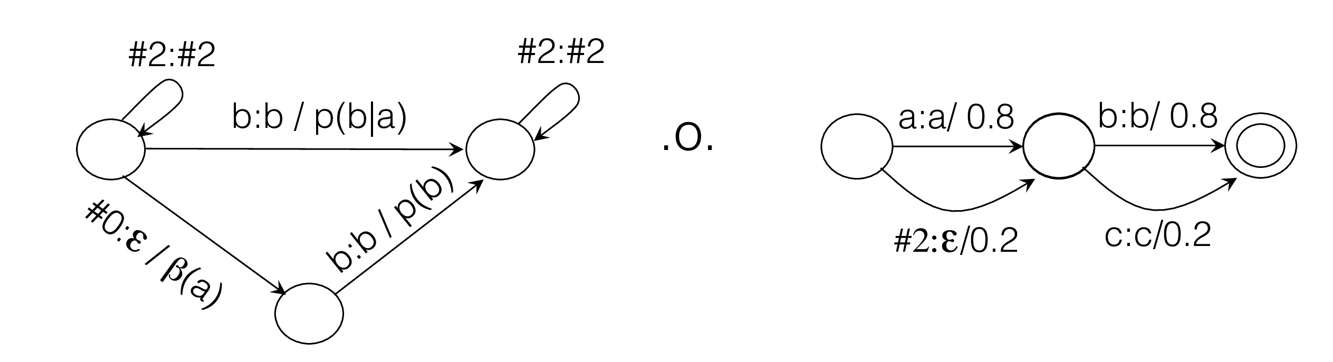
\includegraphics[width=5in]{../figs/liu1.png}}
  \caption{Deletion edges in the probabilistic transcript (edges with
    the special null output symbol, $\epsilon$), required special
    handling in order to use information from a phonotactic language
    model.  As shown, a new type of null symbol, ``\#2'', was invented
    to represent the input for every PT edge with an $\epsilon$ output
    (right).  Such edges were only allowed to match with state
    self-loops, newly added to the language model (left) in order to
    consume such non-events in the transcript.}
  \label{fig:liu1}
\end{figure}

